\documentclass[git]{deltares_manual}

%------------------------------------------------------------------------------
\newcommand{\dfastmi}{\textrm{D-FAST~Morphological~Impact}\xspace}
\newcommand{\dfmi}{\textrm{D-FAST~MI}\xspace}
\newcommand{\dflowfm}{\textrm{D-Flow~FM}\xspace}
\newcommand{\sobek}{\textrm{SOBEK}\xspace}

\hypersetup
{
    pdfauthor   = {Deltares},
    pdftitle    = {\dfastmi},
    pdfkeywords = {Release Notes \dfmi}
}

\begin{document}
\pagestyle{empty}
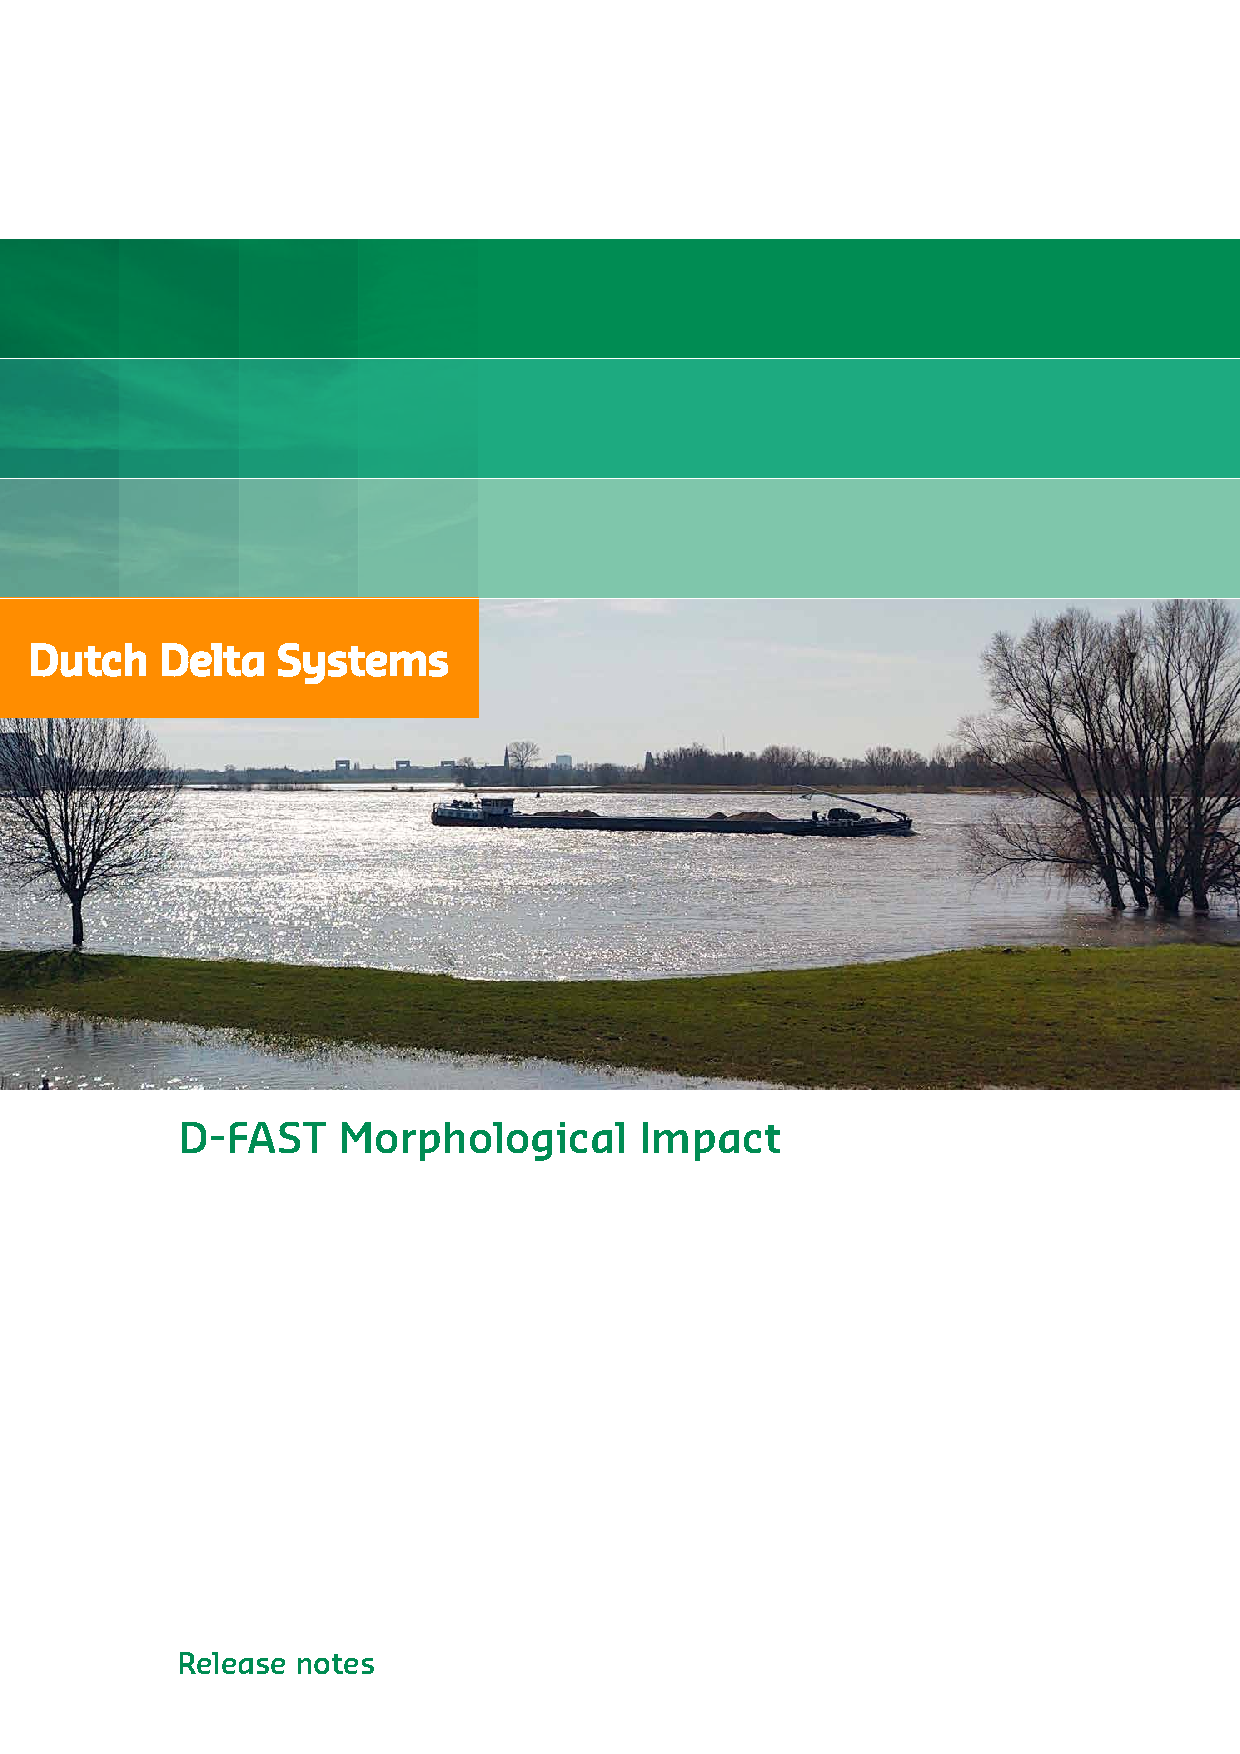
\includepdf[pages=1, offset=72 -70]{cover/D-FAST-omslag-D-FAST Morphological Impact-RN.pdf} % links-rechts past precies
\cleardoublepage
\title{D-FAST\\ Morphological Impact 3.1.0}
\subtitle{}
\manualtype{Release Notes}
%\distribution{Released for: \newline \phantom{M} \dfmi version 3.1 or higher}
\version{\the\year.\the\month}

\author{ }

\setgitdirectory{../.git}
\deltarestitle

%------------------------------------------------------------------------------
\chapter{Introduction}
\section{Release contents}

\begin{tabular}{ll}
Description: & \dfastmi \\
Version: & 3.1.0 \\
Status & release
\end{tabular}

\fbox{%
\parbox{\textwidth}{%
\dfastmi version 3 is the successor of \dfastmi version 2 and WAQMORF.
This new version implements a generalized algorithm for estimating the sedimentation length and the long-term morphological response of the main channel to changes, so-called interventions, in the flood plains.
The tool requires the results of pairs of \dflowfm computations (with and without the intervention) for a given set of flow conditions.
}}

\section{Installation}
\dfastmi is distributed as a plain zip-file.
To install the software, unzip the file into an appropriate location, say \keyw{d:\textbackslash{}App\textbackslash{}dfastmi3}.
Start the software by running \keyw{d:\textbackslash{}App\textbackslash{}dfastmi3\textbackslash{}dfastmi.exe}.
For more details on the run procedure, see the \dfmi User Manual.

\section {Documentation list}
The following documentation is distributed with this release:

\begin{enumerate}
\item \dfastmi User Manual
\item \dfastmi Technical Reference Manual
\end{enumerate}

\chapter{Release summary}
\section{Key changes summary}

The key changes of this completely revised version are:

\begin{itemize}
\item The number of discharge level used for \dfmi analysis has changed from typically 3 to 6.
The discharge levels no longer depend on the characteristics of the interventions.
They are fixed per branch/reach, although you don't have to provide results below the threshold discharge of the intervention.
\item The new analysis algorithm only supports simulation results stored in netCDF UGRID files, such as the \dflowfm map-file.
\item Complete overview of analysis settings included in the report.
\item The tool is no longer supported in the Dutch language.
\item The WAQMORF compatible \keyw{cli} mode is no longer supported.
\item Configuration files of \dfmi version 2 are no longer supported by the GUI.
\end{itemize}

\section{Known issues}

None

\section{Overview of all issues}

An overview of all closed issues since the release of version 2.0.10 is given in the table below.

\begin{longtable}{l|l|p{8cm}}
\caption{List of resolved issues for version 3.1.0} \\
Issue & Type & Description \\ \hline
\endfirsthead
\multicolumn{3}{l}{\textsl{(continued from previous page)}} \\
Issue & Type & Description \\ \hline
\endhead
\hline \multicolumn{3}{r}{\textsl{(continued on next page)}} \\
\endfoot
\endlastfoot 
DFAST-137 & Feature & Support for \dflowfm fourier-files. \\
\end{longtable}

\begin{longtable}{l|l|p{8cm}}
\caption{List of resolved issues for version 3.0.0} \\
Issue & Type & Description \\ \hline
\endfirsthead
\multicolumn{3}{l}{\textsl{(continued from previous page)}} \\
Issue & Type & Description \\ \hline
\endhead
\hline \multicolumn{3}{r}{\textsl{(continued on next page)}} \\
\endfoot
\endlastfoot 
DFAST-211 & Bug & Include LICENSE.md file as referrenced in the Version dialog \\
DFAST-210 & Bug & Mismatch between files reported and files used \\
DFAST-209 & Bug & configuration file should contain one set of keywords \\
DFAST-207 & Improvement & Increase version number in rivers and configuration file to 3.0 to align with major software update \\
DFAST-206 & Bug & Adjust the report of the configuration settings \\
DFAST-205 & Bug & D-FAST MI doesn't write names of simulation files to config file \\
DFAST-203 & Task & Update TC configurations that use CentOS7 to use Alma8 \\
DFAST-202 & Bug & Graphs are not saved to correct location when loading config twice \\
DFAST-201 & Bug & When disabling make figures with save figures enabled, the figure directory stays editable in the GUI \\
DFAST-200 & Bug & App crashes when RiverKM key is not in general section of DFAST MI config file \\
DFAST-199 & Bug & When loading DFast MI configuration and checkbox make plots is set not all plot controls are enabled \\
DFAST-198 & Bug & Retain sections and keys unknown in gui \\
DFAST-197 & Bug & Safely retrieve keys from config \\
DFAST-196 & Bug & QThreshold is not read correctly or not used correctly \\
DFAST-195 & Improvement & Remove second branch discharge location from GUI \\
DFAST-194 & Improvement & Improve performance update branch selection \\
DFAST-193 & Bug & Saving a loaded configuration file for RiverKM and ClosePlot does not result in the same file \\
DFAST-192 & Bug & Crash when saving a configuration file at a different location \\
DFAST-191 & Bug & Crash when saving config file in output directory \\
DFAST-190 & Bug & Resolve Fallout DFAST-123 \\
DFAST-188 & Bug & "Open user manual" option in GUI does not work \\
DFAST-185 & Improvement & improve cognitive complexity of \_clear\_conditions \\
DFAST-181 & Bug & Application crashes when selecting typing text into 'Uitvoer map' field \\
DFAST-180 & Bug & Application crashes when selecting MaakFiguren \\
DFAST-179 & Bug & Load of .cfg causes a crash in the GUI \\
DFAST-178 & Bug & Resolve failing build config on Teamcity \\
DFAST-176 & Task & [Investigate] Problem with teamcity in which tests passed and artifacts are not generated and shown \\
DFAST-175 & Bug & Resolve Fallout DFAST-125  \\
DFAST-174 & Improvement & Refactor gui to MVVM \\
DFAST-170 & Improvement & Write conditions and simulation files to the report file \\
DFAST-169 & Improvement & Write description to the report file \\
DFAST-168 & Improvement & Write basic analysis settings to the report file \\
DFAST-161 & Improvement & Use Select Directory dialog when appropriate \\
DFAST-160 & Improvement & Grey out fields if Q < Q\_threshold \\
DFAST-159 & Improvement & Add a case description \\
DFAST-158 & Improvement & Use D-FAST MI logo in Window bar of GUI \\
DFAST-156 & Bug & [Investigate] Crashing dfastmi application \\
DFAST-148 & Task & Ignore test result directories \\
DFAST-147 & Task & Fix package name in pyproject.toml \\
DFAST-145 & Improvement & Use ConfigParser getint, getfloat, getboolean instead of DFastMIConfigParser \\
DFAST-144 & Bug & crash in line 284 of AnalyserAndReporterDflowfm \\
DFAST-143 & Improvement & verify basic usage of DFAST-MI works without extra admin rights in virtual machine \\
DFAST-142 & Improvement & Update year in D-FAST MI version/about screen to 2024 \\
DFAST-141 & Bug & Resolve small fallout of DFAST-104 \\
DFAST-140 & Task & Refine determine how to align the Rkm values in the reach list \\
DFAST-139 & Improvement & Modify GUI layout \\
DFAST-138 & Improvement & Suppress the command window \\
DFAST-136 & Improvement & Use LookupException when provided language is not as expected \\
DFAST-135 & Improvement & Add coverage html report in Teamcity unit test configuration as result \\
DFAST-133 & Task & Use new logo for DFAST-MI the .exe \\
DFAST-131 & Task & Configure black package for automating formatting \\
DFAST-130 & Task & [Investigate] Using pydantic to replace validation \\
DFAST-129 & Task & [Investigate] Reuse of modules from Hydrolib Core \\
DFAST-127 & Improvement & Include SIG analysis in CI workflow \\
DFAST-126 & Bug & During RiverObject refactoring relinking new functionality is not good connected \\
DFAST-125 & Improvement & Refactor batch.core.py and add/update related tests \\
DFAST-124 & Improvement & Refactor DetectAndPlot.py and add/update related tests \\
DFAST-123 & Improvement & Refactor analyserAndReportDflowfm.py and add/update related tests \\
DFAST-122 & Improvement & Refactor analyserAndReportWaqua.py and add/update related tests \\
DFAST-121 & Improvement & Refactor FileNameRetriever.py and add/update related tests \\
DFAST-120 & Improvement & Refactor ConfigurationChecker.py and add/update related tests \\
DFAST-119 & Improvement & Resolve leftover change from DFAST-115 \\
DFAST-118 & Improvement & Add Distribution test to test that the Gui can startup \\
DFAST-115 & Bug & Resolve dfastmi.exe not starting after gui v2 update \\
DFAST-114 & Improvement & Debug with arguments DFAST in VSCode \\
DFAST-113 & Improvement & Refactor RiversObject and related tests \\
DFAST-112 & Improvement & Refactor RiverParameterData and related tests \\
DFAST-111 & Improvement & Refactor GridOperations and related tests \\
DFAST-110 & Improvement & Refactor FileUtils and related tests \\
DFAST-105 & Improvement & Add a test case using version 2 configuration files \\
DFAST-104 & Improvement & Adapt new structure for batch \\
DFAST-103 & Improvement & [Investigate] Refactoring batch \\
DFAST-102 & Improvement & Improve code coverage of the batch \\
DFAST-99 & Bug & Failing batch file 00 is because it is using wrong river file \\
DFAST-98 & Bug & Signing certificate shows bank erosion instead of morphological impact \\
DFAST-97 & Improvement & Resolve codesmells in kernel.py \\
DFAST-96 & Improvement & Investigate Refactoring IO \\
DFAST-95 & Improvement & [Investigate] Remove or refactor estimate\_sedimentation\_length method \\
DFAST-94 & Improvement & Refactor char\_discharge and char\_times in kernel into a new class \\
DFAST-92 & Improvement & Refactor the main\_computation method in Kernel into the BedLevelCalculator class \\
DFAST-91 & Improvement & Refactor the RiversObject.py \\
DFAST-90 & Improvement & investigate and adapt new structure for IO \\
DFAST-89 & Improvement & investigate and adapt new structure for kernel \\
DFAST-87 & Improvement & Investigate Refactoring Kernel \\
DFAST-86 & Improvement & Refactor unit \& unit test names for IO \\
DFAST-85 & Improvement & Refactor existing unit tests \& unit test names for Kernel \\
DFAST-84 & Improvement & Update nuitka build config with extra information and nofollow-import-to \\
DFAST-83 & Improvement & Update nuitka build config with include-data-files \\
DFAST-82 & Improvement & Update nuitka build config to include icon for .exe \\
DFAST-81 & Improvement & Update nuitka build config to include details/company information \\
DFAST-79 & Improvement & Improve code coverage of the Kernel  \\
DFAST-77 & Improvement & Clean and setup debug and coverage \\
DFAST-76 & Bug & Resolve bug with crash during compute with empty input \\
DFAST-75 & Improvement & Improve code coverage of the IO \\
DFAST-74 & Improvement & Improve code coverage of the IO  \\
DFAST-72 & Improvement & Investigate if github action sonarcloud run is interesting after unit test have been revised \\
DFAST-71 & Improvement & Resolve issue with running the dfastmi.exe \\
DFAST-70 & Task & Add user documentation \\
DFAST-69 & Task & Setup a changelog document for users \\
DFAST-68 & Task & Resolve SonarCloud issues \\
DFAST-67 & Task & Refine API \\
DFAST-66 & Documentation & Document API and publish it on/via the GitHub page \\
DFAST-65 & Improvement & Investigate unit test coverage \\
DFAST-64 & Improvement & Investigate unit tests of gui.py \\
DFAST-63 & Improvement & Investigate unit tests of cmd.py \\
DFAST-62 & Improvement & Investigate unit tests of kernel.py \\
DFAST-61 & Improvement & Investigate unit tests of io.py \\
DFAST-60 & Improvement &  Investigate unit tests of cli.py \\
DFAST-59 & Improvement & Investigate unit tests of batch.py \\
DFAST-58 & Improvement & Update unit tests to also be able to debug through the tests \\
DFAST-49 & Improvement & Update gui to add new features \\
DFAST-48 & Improvement & Implement acceptation tests \\
DFAST-47 & Improvement & Update batch tests \\
DFAST-46 & Improvement & Update unit tests \\
DFAST-45 & Improvement & Merge feature/developments-2021 into the master branch \\
DFAST-44 & Improvement & Create developer starting guide \\
DFAST-43 & Improvement & [Investigate] Multiple language support \\
DFAST-42 & Improvement & Setup Sonarcloud for D-Fast MI \\
DFAST-40 & Task & [Investigation] Steps needed for professionalization D-FAST MI \\
DFAST-35 & Task & Consider implementing SonarCloud  \\
\end{longtable}

%------------------------------------------------------------------------------
\pagestyle{empty}
\cleardoublepage
\mbox{}
\includepdf[pages=2, offset=-72 -70]{cover/D-FAST-omslag-D-FAST Morphological Impact-RN.pdf} % links-rechts past precies
\end{document}
